%!TEX root = ../main.tex

\section{Results}
\subsection{Study Inclusion}
Figure XXX shows the results of the systematic process to identify, screen, assess, and select studies for inclusion according to the PRISMA guidelines. 

During the identification phase, XXXX studies from the four different Web-based sources (Scopus, Web of Science (WoS), PsycINFO, and PubMed, using com), which we reduced to YYY after removing duplicates. After initial screening (based on title and abstract), we retained ZZZ articles. The eligibility assessment (based on full article) resulted in a final set of 120 papers. More details can be found in Figure XXX.


\subsection{Study Characteristics}

Presenting all eligible papers in the form of a table to summarize main characteristics + citation them is mandatory.

 % ---------------------------------------------------------
\subsection{Target Conditions and Hardware Platforms}
Figure \ref{fig:disorders_devices} shows the distribution of research over time, sub-classified according to technological platforms used and mental disorders addressed. 

\begin{figure}[H]
    \centering
    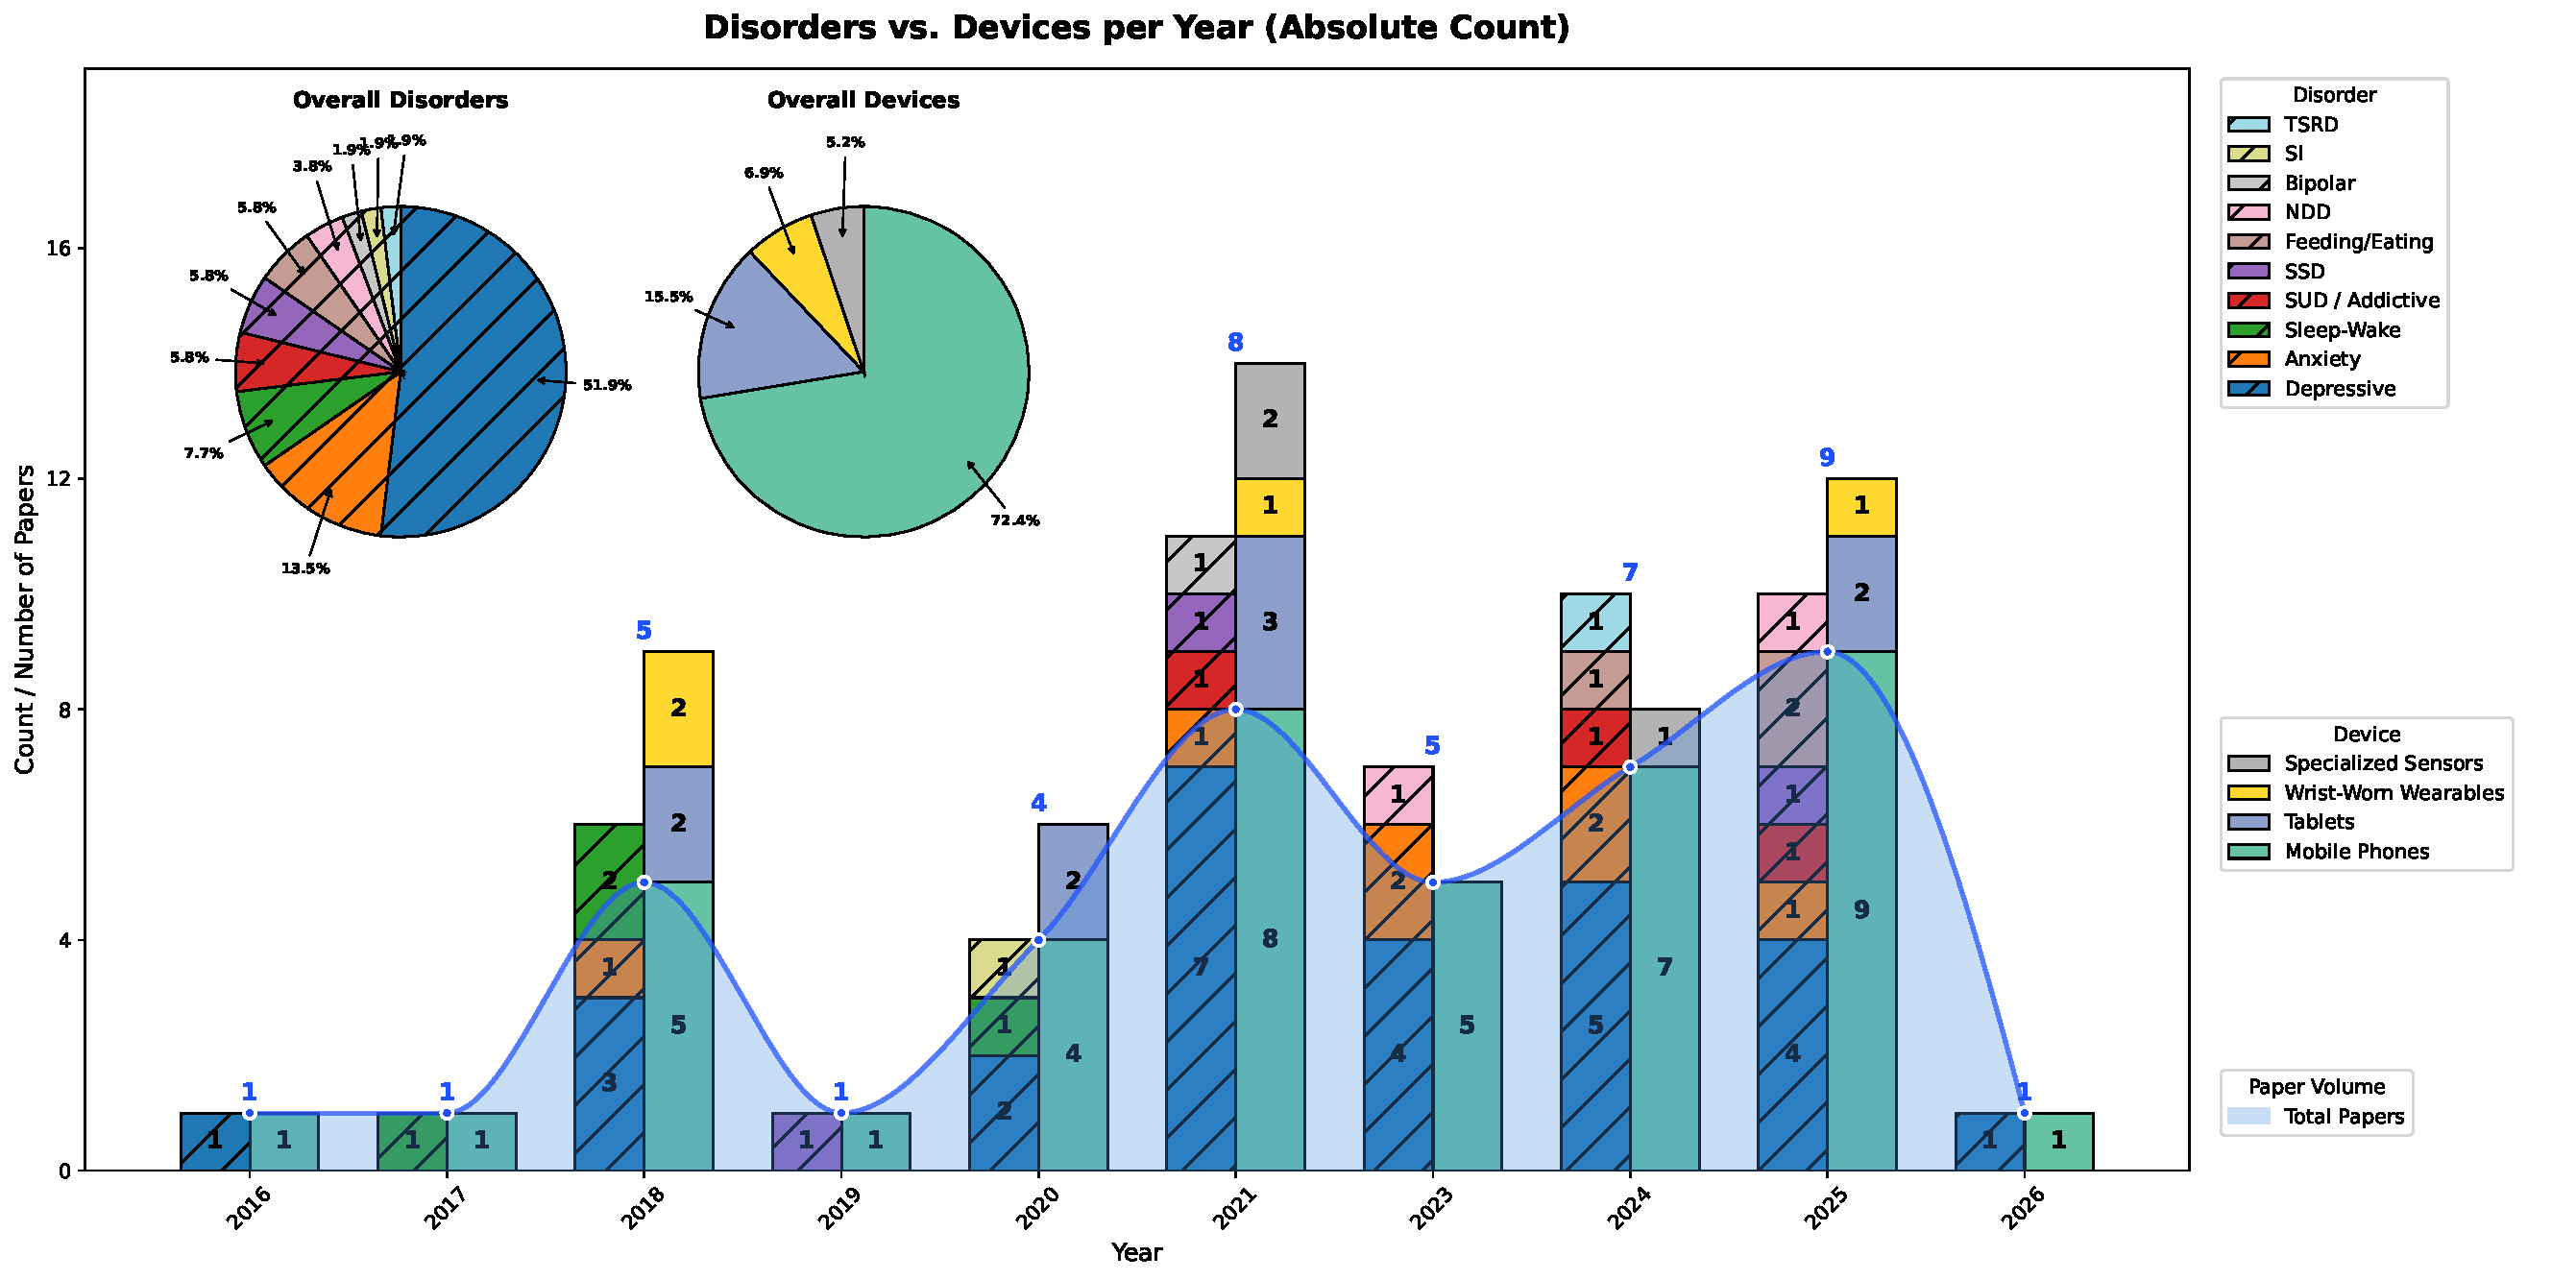
\includegraphics[width=0.95\textwidth]{sections/charts/DisordersDevicesHisto.pdf}
    \caption{Joint longitudinal distribution of included papers categorized by targeted mental disorders and deployed hardware platforms.}
    \label{fig:disorders_devices}
\end{figure}

Overall, the number of publications sharply increased since 2020-2021, coinciding with the start of the coronavirus pandemic, with peaks in 2021 and 2025 (note that 2026 is incomplete). Research efforts are heavily clustered around high-prevalence internalizing disorders, particularly depression and anxiety (66,0\% combined), whose relevant proportion remained equal after the 2020-2021 increase. Other disorders, particularly Substance Use Disorders (SUD/Addictive), Somatic Symptoms Disorder (SSD), Sleep-Wake Disorders and Bipolar Disorder are already sporadically addressed before 2020, with a further increase in their coverage and branching out into other mental disorders since 2020.
%Other classes of conditions, namely Substance Use Disorders (SUD/Addictive), Trauma- and Stressor-Related Disorders (TSRD), Neurodevelopmental Disorders (NDD), and Bipolar Disorder, make up significantly smaller shares, and are found in increasing amount since 2020, thus indicating that context-aware intervention strategies are just starting to branch out into non-prevalent internalizing disorders. 
Conditions of Suicidal Ideation (SI), Feeding/Eating, Sleep-Wake, and Somatic Symptom Disorders (SSD) appear scarcely represented in the examined timeframe.

As for hardware platforms employed, mobile phones constitute the technological substrate for the overwhelming majority of interventions, due to their omnipresence, accessibility and their variety of available sensors. Wrist-worn wearables occupy the second place on the list of platforms; however, their prevalence grows noticeably from 2020 onwards, likely owing to the general growth of consumer market demand for devices such as smartwatches and fitness trackers. The third group comprises tablets and displays, which are used occasionally. Specialized/clinical devices, XR technologies, and proximity sensors are rarely employed in the field.

% ---------------------------------------------------------
\subsection{Captured Contextual Data:}
To minimize user interaction friction, modern intervention architectures increasingly rely on background diagnostic logging to establish context. [cite: 14]

\begin{figure}[H]
    \centering
    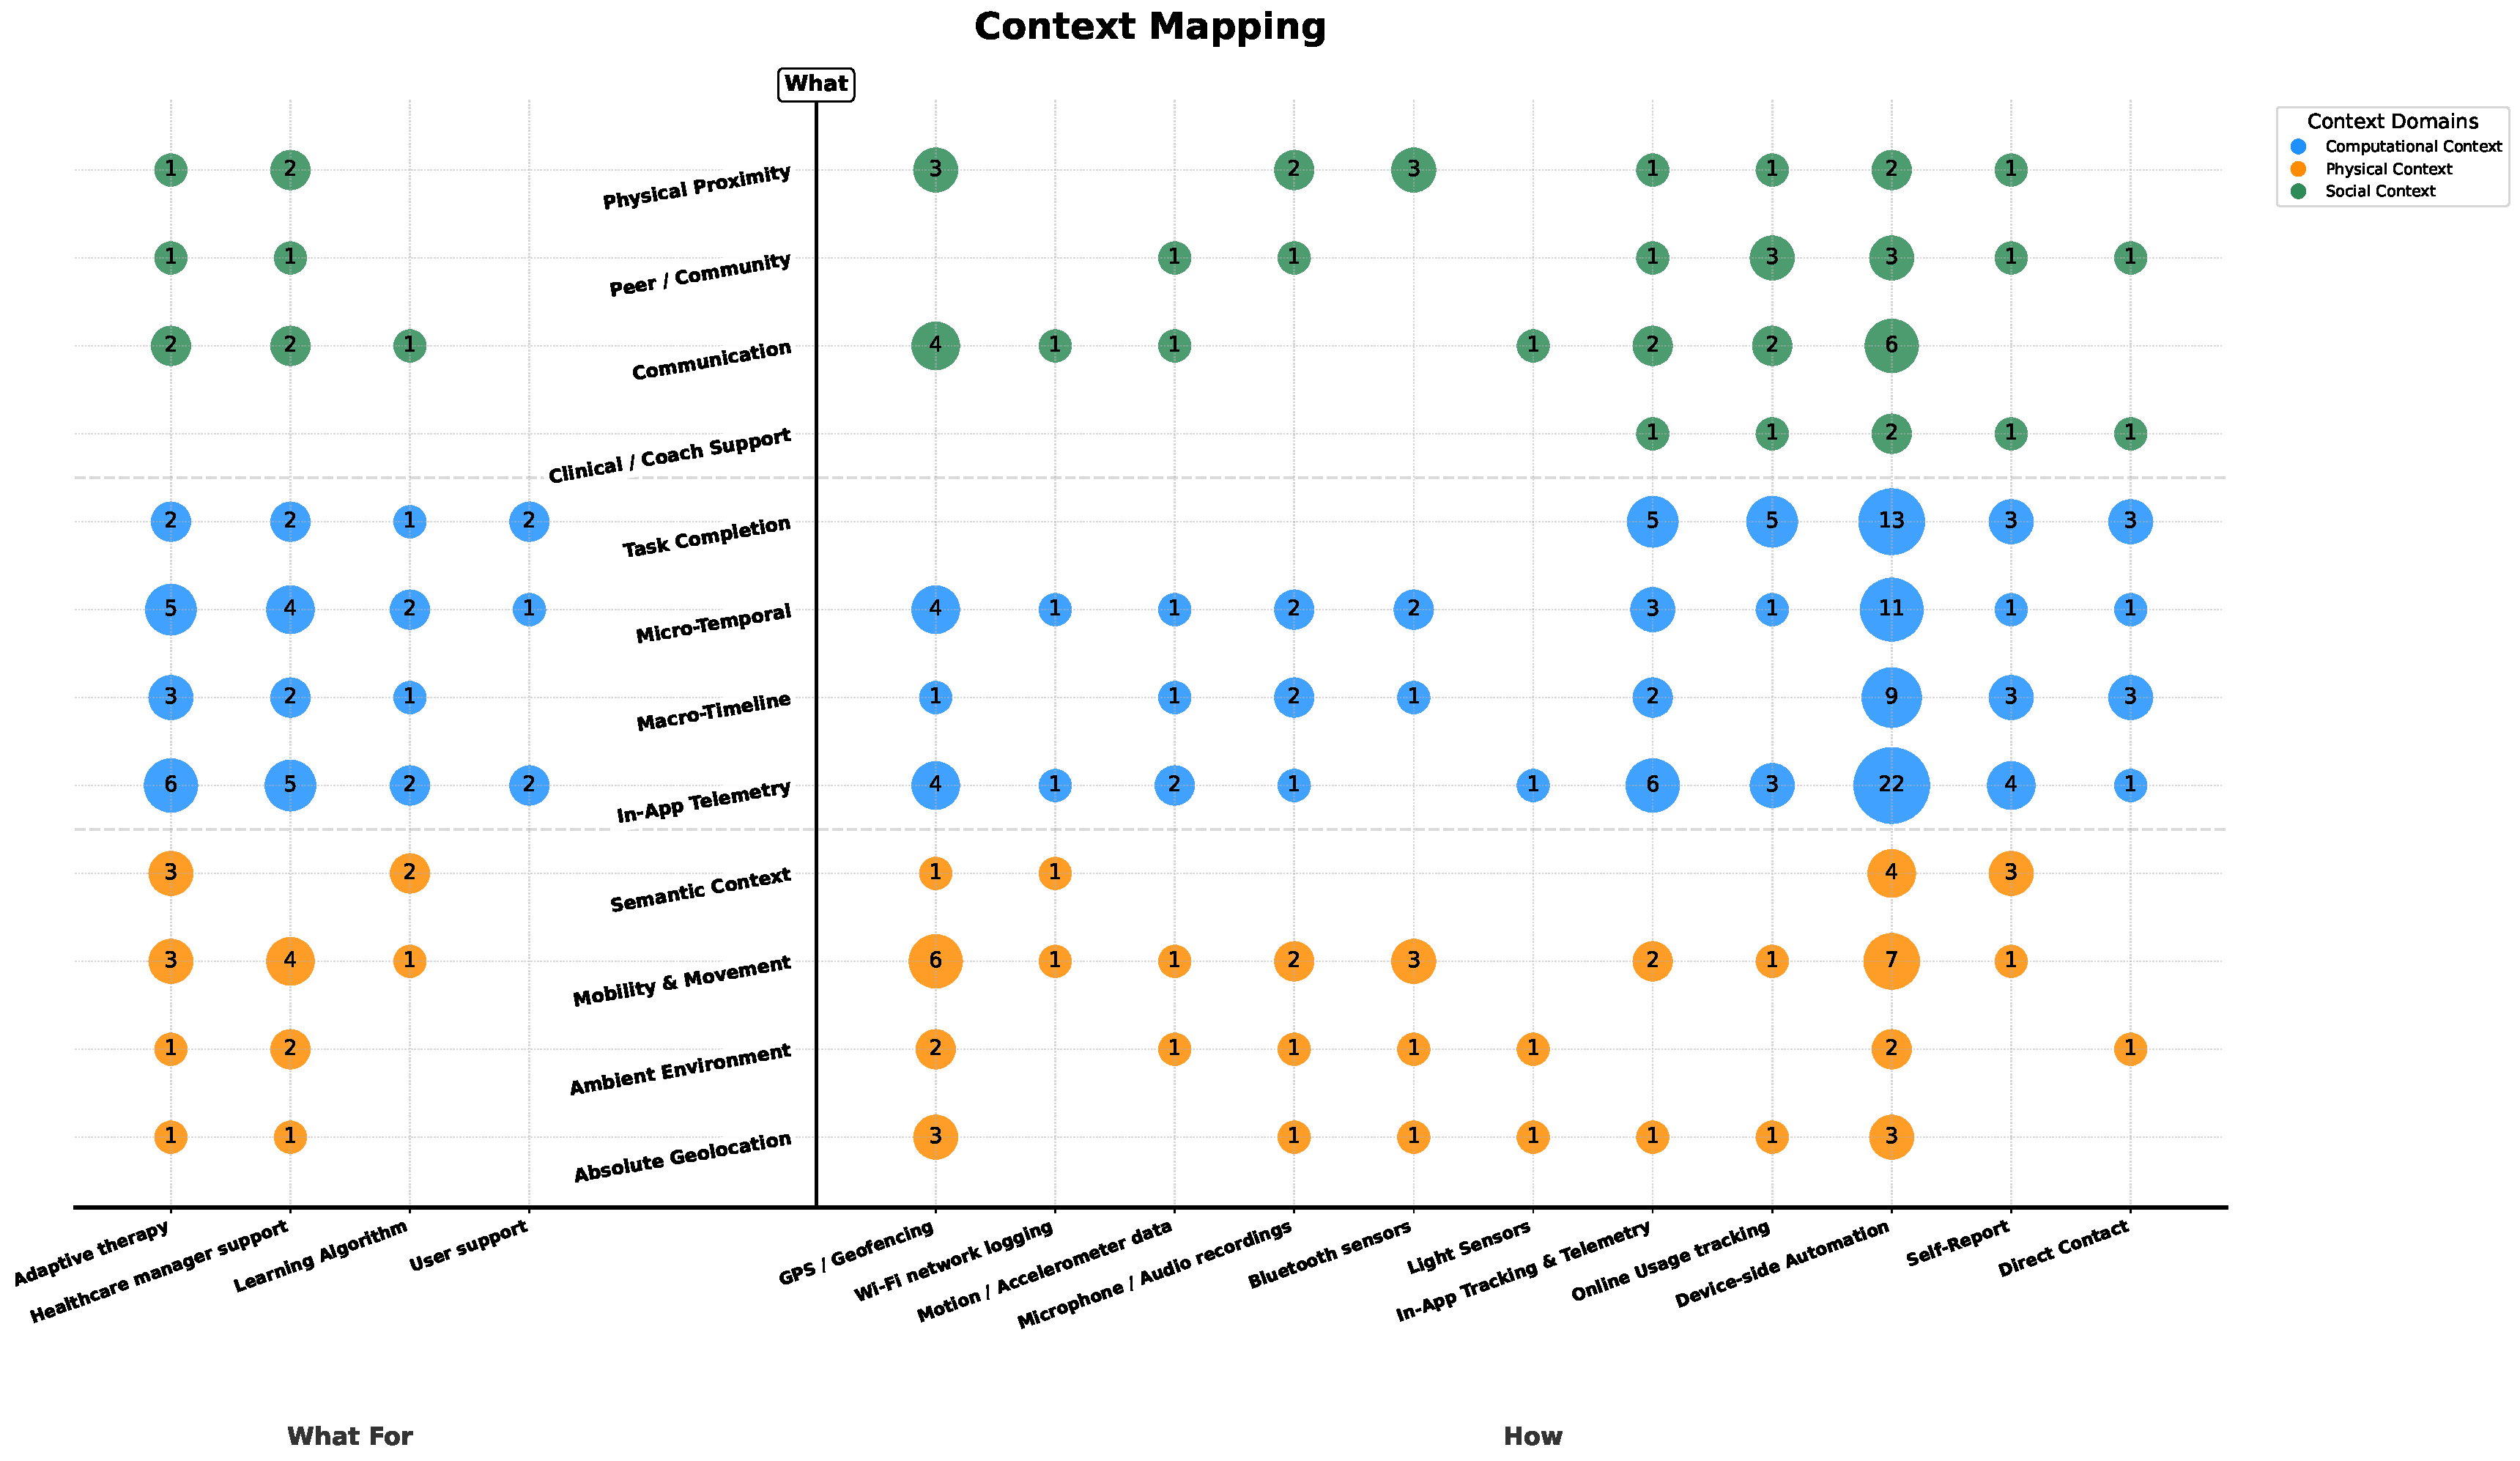
\includegraphics[width=1\textwidth]{sections/charts/bubbleChart.pdf}
    \label{fig:bubble_matrix}
\end{figure}

In order to minimize interaction cost, the architecture of contemporary interventions is being optimized to use background diagnostic logging to create a context awareness. As seen from the Context Mapping in Figure~\ref{fig:bubble_matrix}, the distribution of contextual variables among 120 included interventions remains rather biased with Computing Context accounting for the majority of captured contextual factors (65\% of all contextual variables), Physical Context (18\%) and Social Context (17\%).

Speaking of Computing Context, the most prominent subcategory is In-App Telemetry (APP) making up to 38\%, followed by Task Completion metrics (TSK -- 25\%), Micro-Temporal patterns (MIC -- 20\%) and Macro-Timeline behavioral rhythms (MAC -- 18\%). Such an overwhelming focus on computational and behavioral data could be explained by easy accessibility of native data streams as well as low instrumentational burden imposed on the user.

In terms of Physical Context, the most utilized subcategories include Mobility and Movement data (MOB -- 28\%) and Semantic Context (SEM -- 26\%) followed by Absolute Geolocation (ABS -- 19\%) and Ambient Environment data (AMB -- 14\%). Activity and Routine (ACT -- 11\%) is represented by a slightly smaller portion of data, Virtual and Simulated environments (VIR -- 2\%) by a tiny minority of XR-based interventions.

Peer and Community signals (PEER -- 35\%) and Communication metrics (COM -- 25\%) prevail within the Social Context domain along with Clinical or Coach support indicators (CLIN -- 21\%). The least significant subcategory is represented by Physical Proximity sensors (PROX -- 19\%) typically used via Bluetooth/Wi-Fi scanning. Privacy and instrumentation issues could explain their underrepresentation.

From the bubble matrix above (Figure~\ref{fig:bubble_matrix}), one can deduce that adaptive therapy/user support is the most popular application area of contextual data followed by healthcare manager support and learning algorithms that make use of a limited subset of contextual signals such as APP, MIC and MOB subcategories.

\begin{figure}[H]
    \centering
    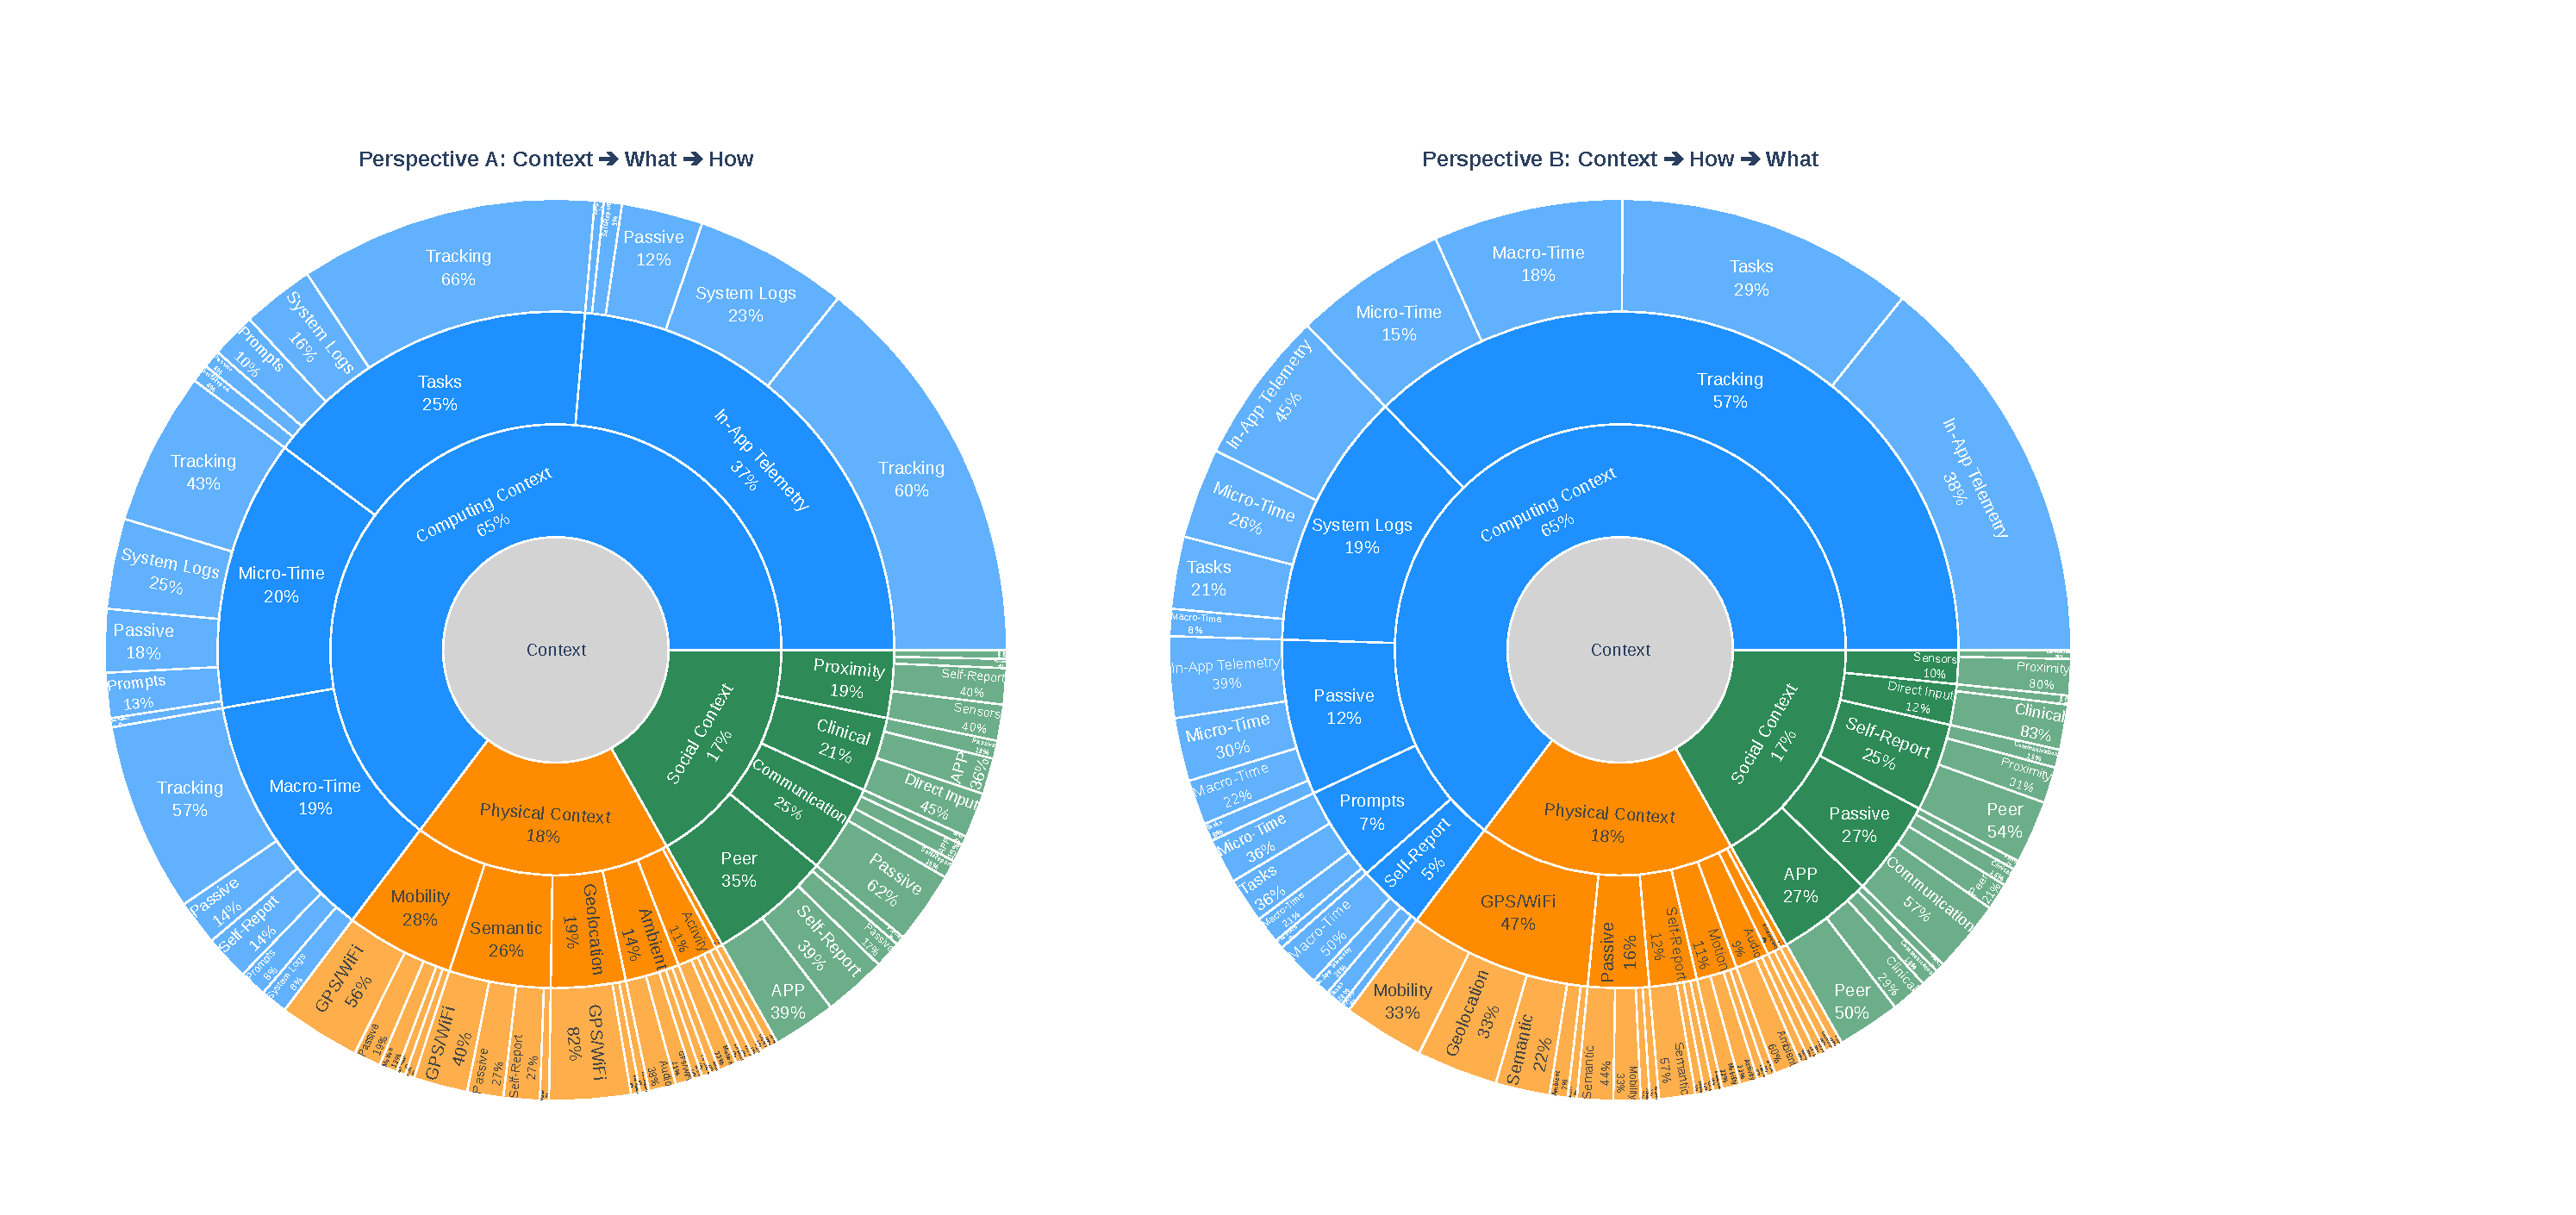
\includegraphics[width=0.85\textwidth]{sections/charts/DualSunburst.pdf}
    \caption{Distribution of technical data collection modalities across active and passive sensing mechanisms.}
    \label{fig:technical_modalities}
\end{figure}


% ---------------------------------------------------------
\subsection{Inerventions mechanisms and classifcation}
\begin{figure}[H]
    \centering
    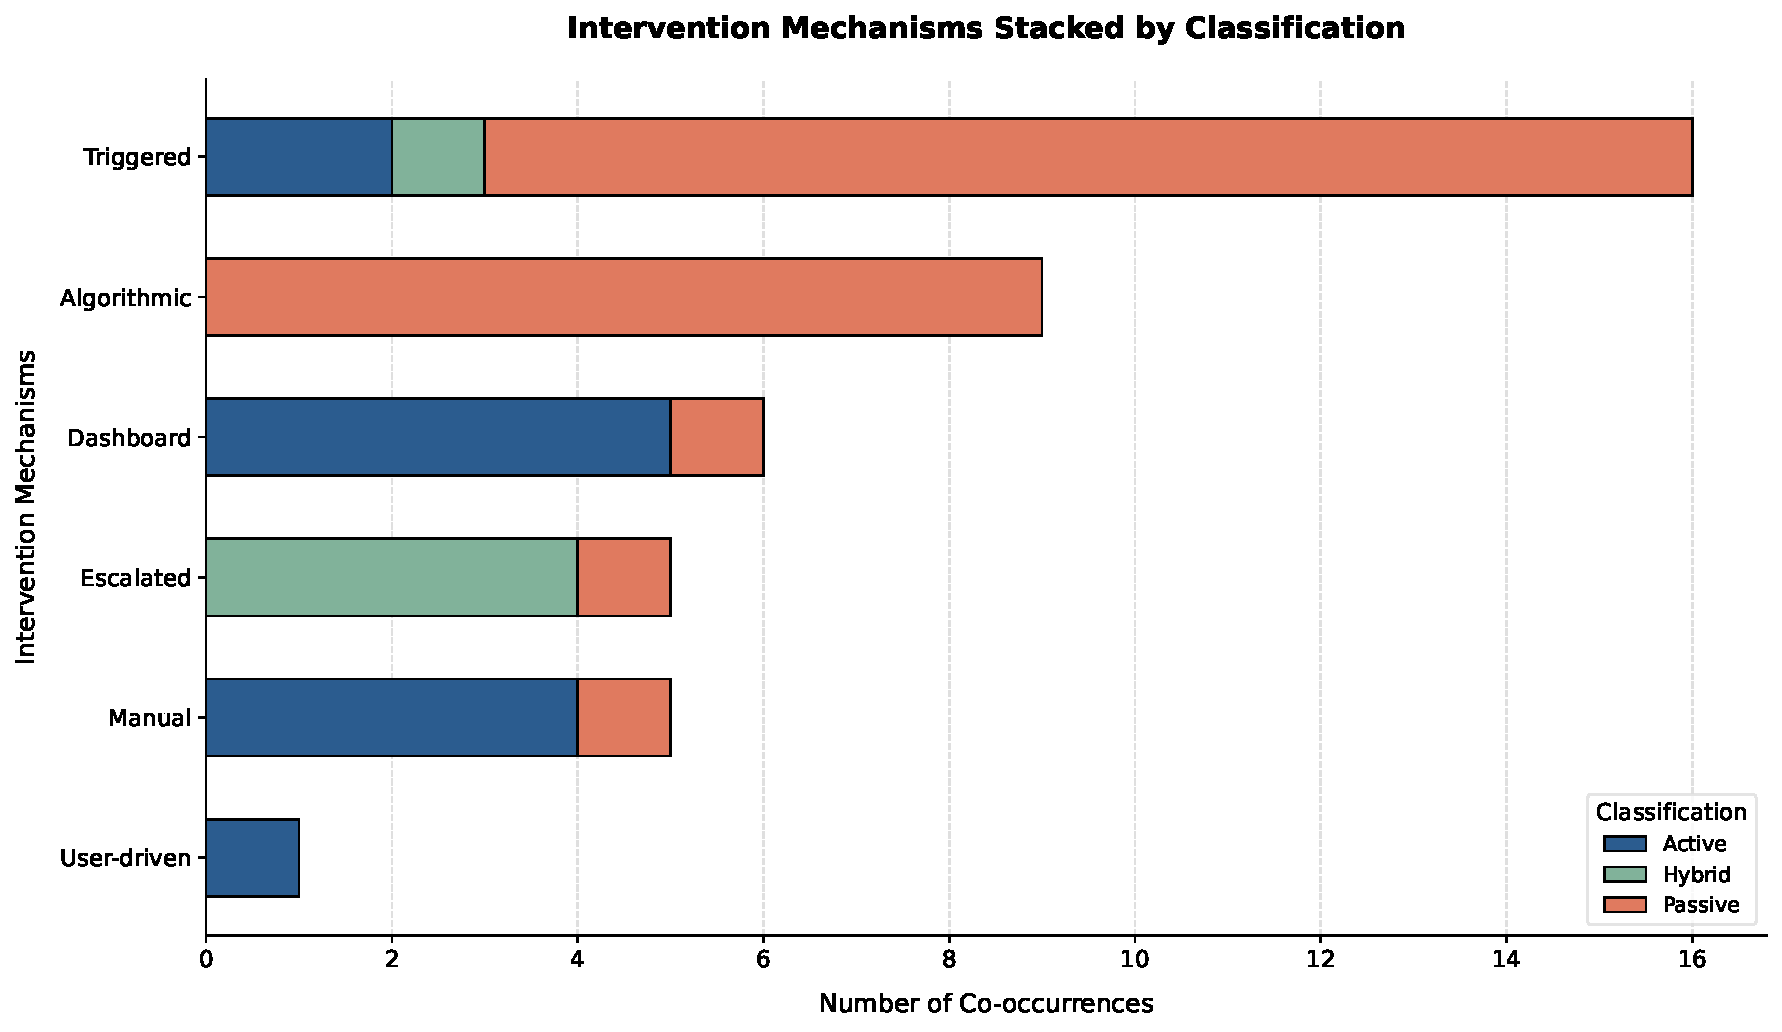
\includegraphics[width=0.85\textwidth]{sections/charts/mechanismClassificationStacked.pdf}
    \caption{Distribution of intervention mechanisms stacked by operational classification.}
    \label{fig:intervention_mechanisms_stacked}
\end{figure}

As evident from Figure~\ref{fig:intervention_mechanisms_stacked}, there is considerable variation in both co-occurrence frequencies and operational characteristics among the six identified intervention mechanisms. This variation reveals a clear structural divide between automated and human-mediated delivery architectures. The classifications shown in the figure describe how intervention delivery is operationalized: \textit{Active} interventions involve direct modification of treatment through user or clinician actions within the application, \textit{Passive} interventions operate automatically without requiring user engagement, and \textit{Hybrid} interventions combine automated detection with subsequent human involvement.

The most frequently occurring mechanism of intervention found in all the studied articles is the \textit{Triggered} interventions that rely on pre-defined rules for automatic delivery of alerts, prompts or recommendations depending on whether certain contextual conditions have been met. It is the most frequently occurring mechanism out of the six and is mostly associated with the Passive category, which suggests that most of the context-based interventions are delivered automatically, without any effort of the users' side. Only a few examples of the Triggered interventions fall into the category of Hybrid, while the Active interventions are almost not used at all.

The second most common mechanism is \textit{Algorithmic}. Unlike simple rule-based triggering, Algorithmic interventions employ dynamic decision logic, predictive models, or machine learning algorithms to analyze continuously collected contextual information and adapt intervention delivery accordingly. Similar to Triggered interventions, Algorithmic approaches are heavily concentrated within the Passive classification, reflecting the prevalence of automated decision-making systems that operate with minimal human involvement.

In contrast, \textit{Dashboard}-based interventions are characterized by a predominance of Active classifications. Dashboard mechanisms provide clinicians, healthcare professionals, or care managers with visual representations of aggregated patient data that support clinical review and decision-making. The Active nature of these interventions reflects the requirement for a human actor to interpret the information presented and determine whether intervention adjustments are necessary.

A comparable trend is observed for \textit{Manual} interventions. These mechanisms involve healthcare staff or study personnel actively monitoring participant information and initiating contact or support when appropriate. Although Manual interventions occur less frequently than Dashboard-based approaches, they also exhibit a strong tendency toward the Active classification because intervention delivery depends primarily on human judgment and action.

\textit{Escalated} interventions possess their own unique set of characteristics, where most are classified as being a Hybrid type. In such systems, an automated monitoring process constantly checks preset thresholds or risks, triggering an alarm whenever the criteria for intervention are met. Nevertheless, rather than implementing interventions directly, the system leaves the task to a doctor, who then decides on the appropriate course of action.

Finally, \textit{User-driven} interventions represent the least frequent mechanism and are exclusively associated with the Active classification. These interventions depend on participants intentionally interacting with the system to access support, initiate activities, or request assistance. As intervention initiation is entirely dependent on user action and does not involve automated background processes, User-driven approaches are inherently Active.

Overall, the results suggest a bimodal structure of intervention design. One pole is represented by passive and highly automated approaches, primarily embodied by the Triggered and Algorithmic mechanisms, where intervention delivery occurs with little or no human involvement. The opposite pole consists of active and human-mediated approaches, represented by Dashboard, Manual, and User-driven interventions, all of which rely on human judgment or participant engagement. Escalated interventions occupy an intermediate position, combining automated detection with human oversight and therefore bridging the two delivery paradigms.

% ---------------------------------------------------------
\subsection{Studies Designs and Evaluation Metrics}
\begin{figure}[H]
    \centering
    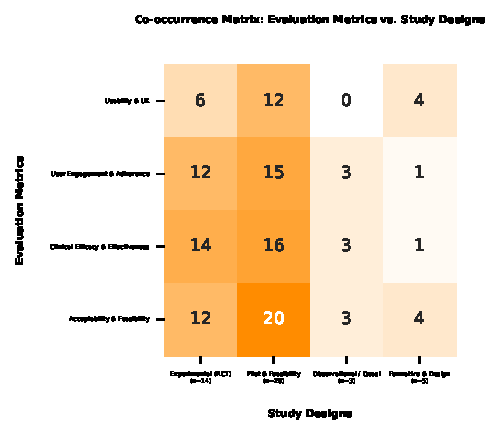
\includegraphics[width=0.85\textwidth]{sections/charts/EMSTDheatmap.pdf}
    \caption{Distribution of study designs and evaluation metrics.}
    \label{fig:metrics_designs_heatmap}
\end{figure}

Figure~\ref{fig:metrics_designs_heatmap} provides an overview of the types of study designs and evaluation metrics used in the selected literature. According to the results of the analysis, Pilot and Feasibility study designs were the most common ones among the considered articles ($n = 49$; 43.8\% of classified studies). Experimental Randomized Controlled Trials (RCTs) came second in terms of prevalence ($n = 40$; 35.7\%). Formative and Design studies ($n = 12$; 10.7\%) and Observational or Quasi-experimental studies ($n = 11$; 9.8\%) were relatively uncommon.

As far as evaluation metrics are concerned, the following criteria proved to be the most popular ones among researchers. First, Acceptability and Feasibility measures appeared in all Pilot and Feasibility studies ($n = 49$) and in many RCTs ($n = 33$; 82.5\%) and Observational studies ($n = 9$; 81.8\%). Second, Clinical Efficacy and Effectiveness, and User Engagement and Adherence were widely applied criteria in RCTs ($n = 38$; 95.0\% and $n = 35$; 87.5\%, respectively) and Observational studies ($n = 10$; 90.9\% and $n = 11$; 100\%, respectively). However, Usability and UX evaluation criteria were limited to Pilot and Feasibility ($n = 36$; 73.5\%) and Formative and Design studies ($n = 7$; 58.3\%) and relatively unpopular in RCTs ($n = 18$; 45.0\%) and Observational studies ($n = 2$; 18.2\%).

Thus, one can clearly observe a certain division of the methodology used. The former focuses on user-centered interaction design and feasibility, and the latter stresses clinical and engagement measures.